\section{Evaluation}
We conducted a user-centered evaluation of SenseMap in a naturalistic work setting to explore its effectiveness in providing the desired support for sensemaking through the \emph{collect -- curate -- communicate} process. 

\subsection{Method}
%goal, overview setup
We recruited five participants who were all working as junior designers and engineers in an innovation center. The participants were all introduced to the tool, trained in its operation and given thirty minutes to try out the tool with support, before being given the task. Each participant installed the tool on their own device; all participants were using laptops (three Apple Macs and two Windows) -- and one participant had a second larger monitor connected. The participants conducted the task in their normal working environment (\autoref{fig:sm-evaluation-settings}) over a two-hour period.

\begin{figure}
	\centering
	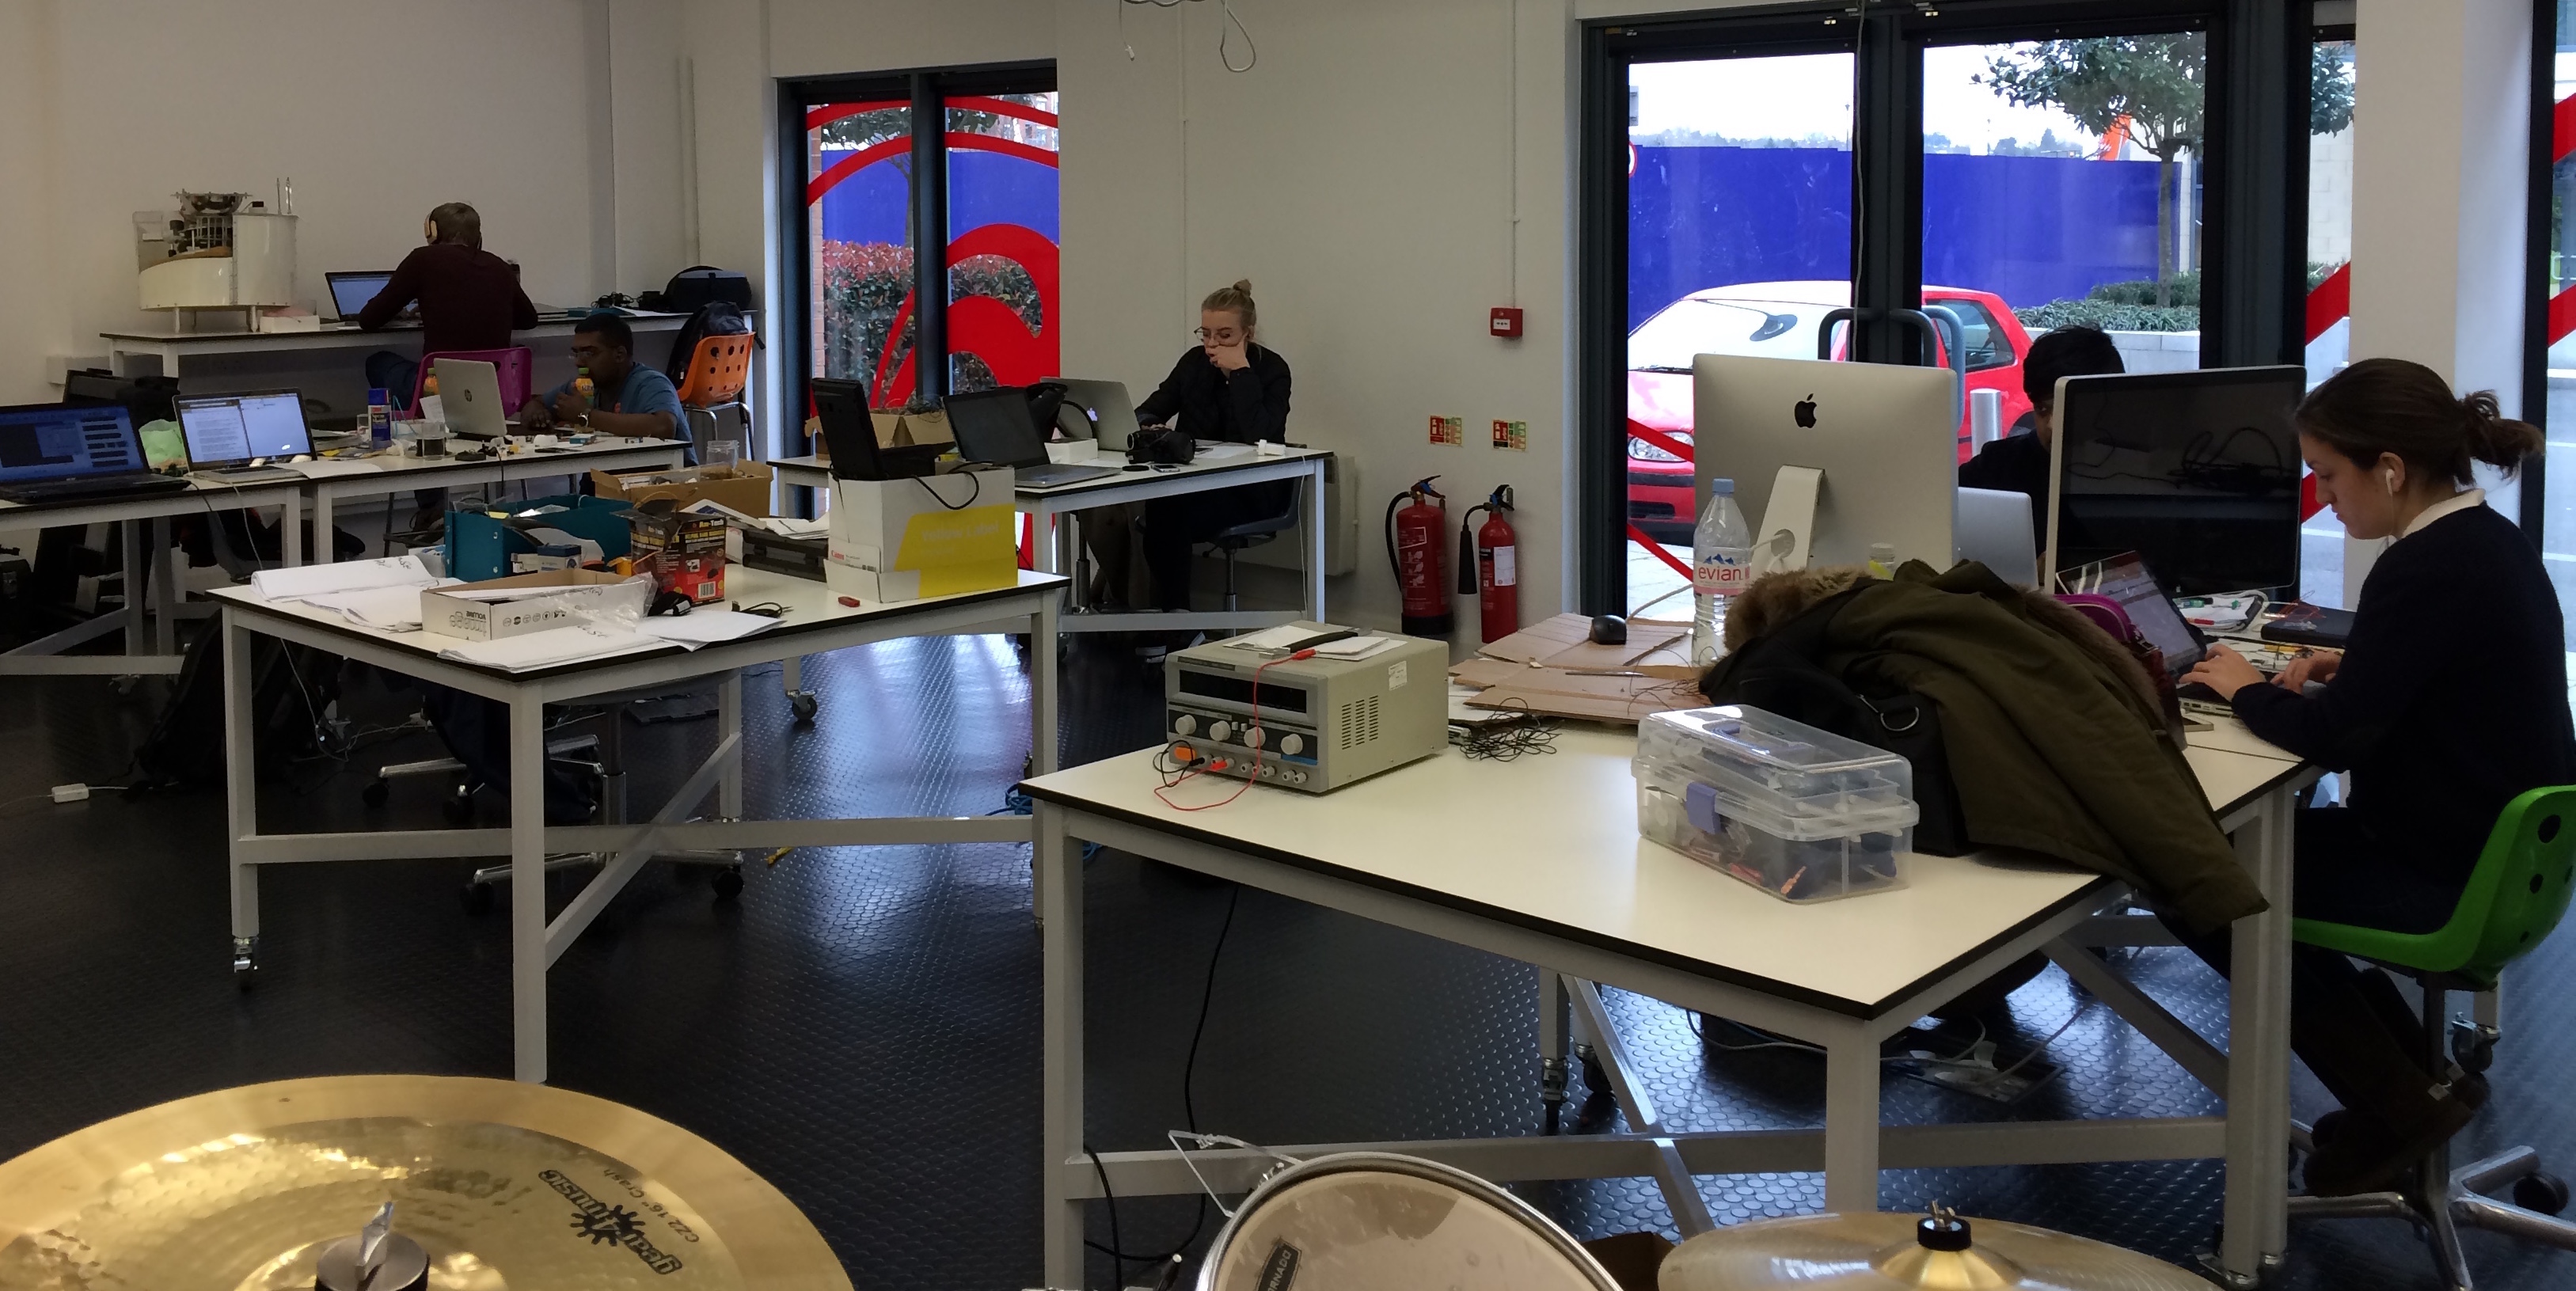
\includegraphics[width=\linewidth]{evaluation-settings.jpeg}
	\caption[Naturalistic work setting in the evaluation]{The working environment of the participants, which was also used in the evaluation to ensure a naturalistic work setting.}
	\label{fig:sm-evaluation-settings}
\end{figure}

%task
The task was devised to reflect normal work activities for these participants in the early research phases of an innovation project. We focused the task on technology selection and deployment, requiring them to collect and curate information on a variety of interrelated areas and then to communicate their findings. Participants were given the task in written form, and it was discussed to clarify any points of confusion or ambiguity. They were asked to complete the following task while using SenseMap to record and present their findings: ``We need to use accelerometers to measure movement intensity in ambulatory subjects and naturalistic settings, for up to 1 week. We need to find out about (in no order of priority): prior art, placement of devices, algorithms, commercial products and APIs, bespoke approaches, and anything else you feel relevant.''

At the end of the two-hour period we conducted an individual, semi-structured interview with each of the five participants. The participants were asked to present their findings, describe the process that they used to reach these findings using SenseMap, and to reflect upon their experience. We also collected interaction logs to explore how participants used SenseMap in their sensemaking activities over time including the timing (when), content (what) and position (where). All sensemaking features supported by SenseMap were captured such as highlighting and annotation in the browser, relevance assessment in the history map, and node movement in the knowledge map. Other standard interaction in the browser including window focus, lost and mouse, keyboard events were also captured.

\subsection{Data Analysis}

\subsubsection{Quantitative Features}
The quantitative data showed two distinct engagement profiles; i.e., how the participants engaged in the sensemaking process and interacted with SenseMap. \autoref{table:knowledge} shows the complexity of knowledge maps produced by all participants, indicating how much they were engaged with the tool. Also, \autoref{fig:evaluation-curation-histogram} shows the histogram of curation activities for all participants, allowing us to understand when the participants were most engaged with the tool and what they were doing.

\begin{table}
	\centering
	\sffamily\small
	\caption{Knowledge Map produced by participants.}
	\label{table:knowledge}
	\begin{tabular}{ccc}
		\toprule
		\textbf{Participant} & \textbf{Number of nodes} & \textbf{Number of links} \\
		\midrule
		P1 & 10 & 12 \\
		P2 & 26 & 26 \\
		P3 & 6 & 7 \\
		P4 & 5 & 2 \\
		P5 & 35 & 35 \\
		\bottomrule
	\end{tabular}
\end{table}

\begin{figure}
	\centering
	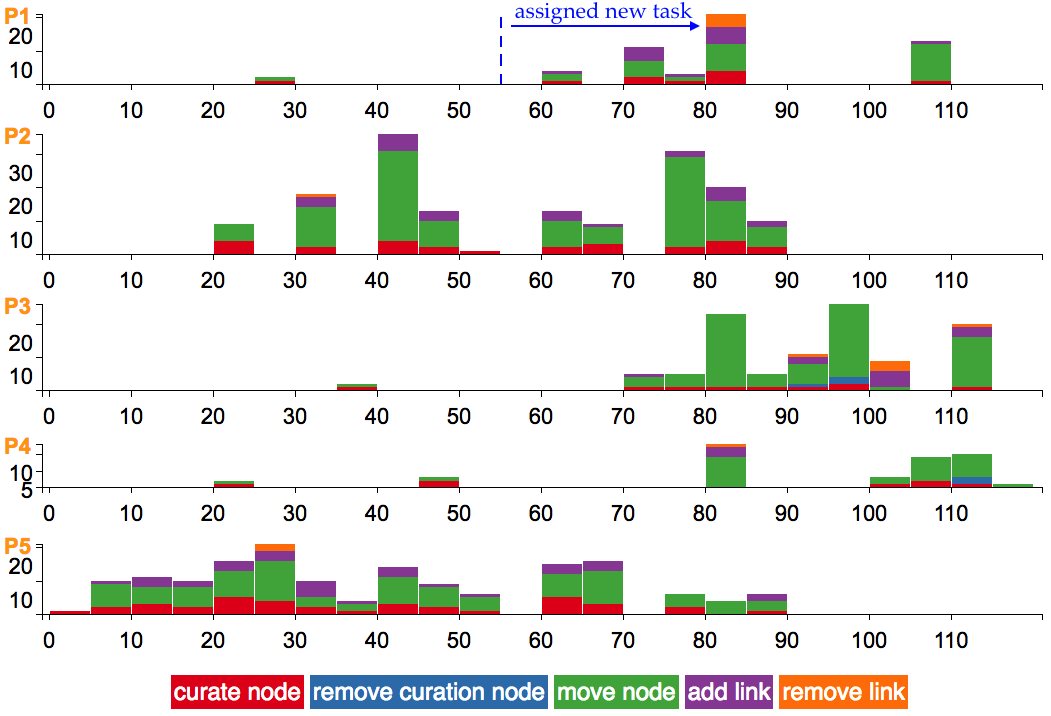
\includegraphics[width=\linewidth]{evaluation-curation-histogram}
	\caption[A histogram of curation activities for all participants]{A histogram of curation activities for all participants, with each bin spanning  5 minutes. Vertical axis shows the number of times the activities were performed.}
	\label{fig:evaluation-curation-histogram}
\end{figure}

\paragraph{High Engagement}
P5 was the first to curate and had the most detailed knowledge map with 35 nodes and 35 links. P2 had a similar profile with early and regular interaction with their window contents. P2 had the second most detailed knowledge map with 26 nodes and 26 links (\autoref{fig:sm-overview}C shows part of it). P1 began the trial with uncertainty due to a lack of technical knowledge of the task. The task was contextualized for P1 helping him to relate it more closely to his expertise. P1 began productive engagement with SenseMap at a later stage resulting in a similar engagement profile to P2 but compressed into a shorter timeframe (starting after around 55 minutes). P1 had the third most detailed knowledge map with 10 nodes and 12 links even though he only spent his second hour for the task. These participants share the same pattern --  \textit{curate early, curate often} -- and it relates to the interplay between collect and curate in our sensemaking model, through refining searches and extending the schema.

\paragraph{Low Engagement}
P3 did some minor curation activities early in the sensemaking process, but there was a considerable rise in the last third of the task time. There were only 6 nodes and 7 links in the final knowledge map with an indeterminate linking structure.

P4 did some minor curation activities with a short focus after an hour and more toward the end of the task. P4's interaction profile is notable for long and frequent periods of inactivity. P4 had only 5 nodes and 2 links in their final knowledge map with an indeterminate linking structure (\autoref{fig:Magda}).

\begin{figure}
	\centering
	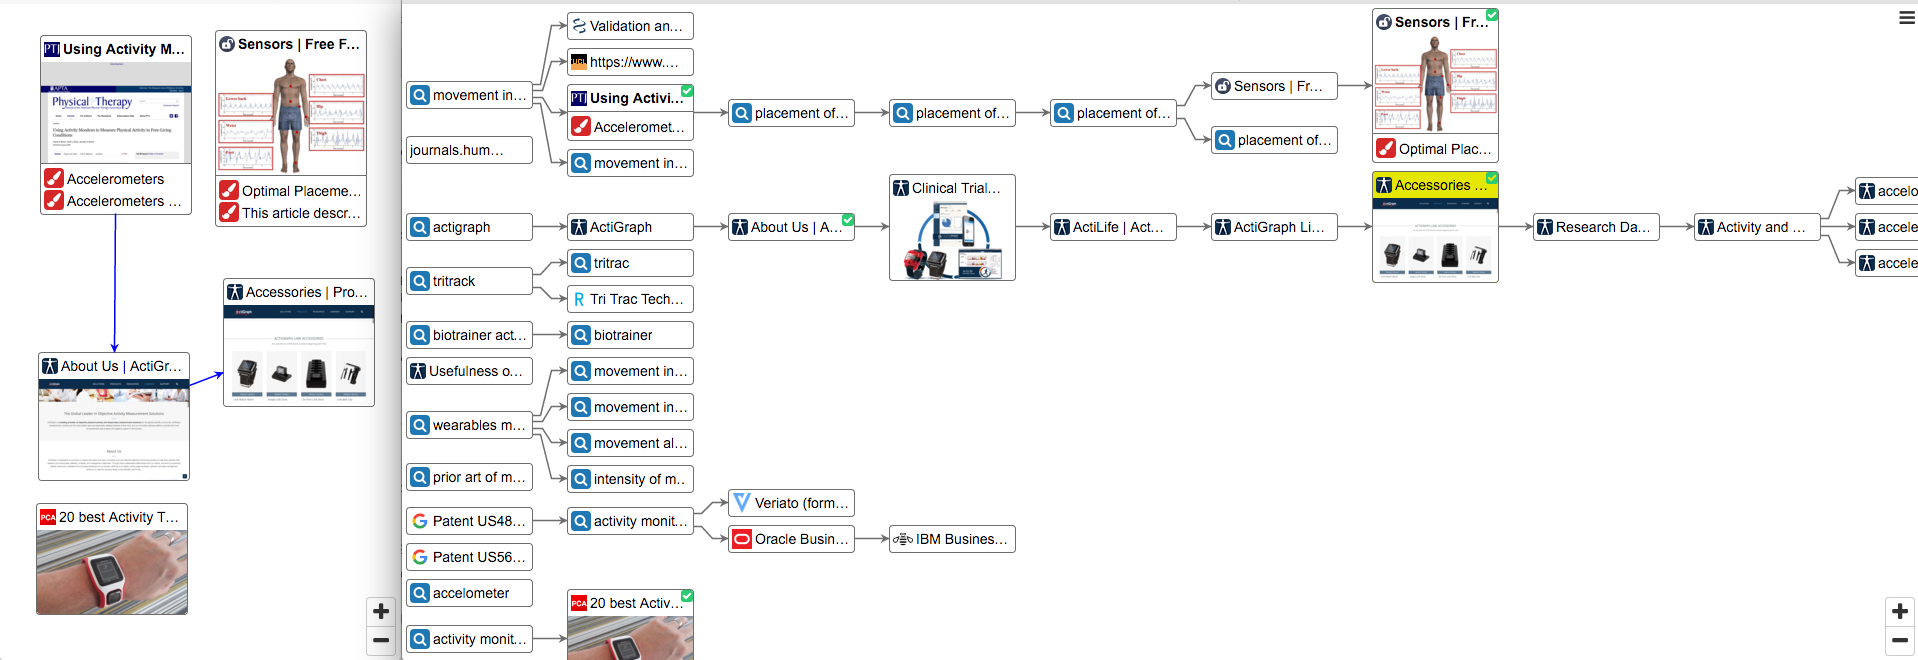
\includegraphics[width=\linewidth]{screenshots-evaluation/P4-Magda}
	\caption[Knowledge map and history map of P4]{P4: Knowledge Map (left) and History Map (right). P4 successfully moved a key document into the curation space, but subsequent schema is scant.}
	\label{fig:Magda}
\end{figure}

\subsubsection{Qualitative Features}

\paragraph{F1 -- Communication}
Did the participants use the knowledge map to communicate their findings? Had they successfully curated their schema through clusters, linked branches or other coherent structures? Had they constructed a narrative to explain their schemas?

\textbf{Positive: P1, P2, P5}. All had arranged their detailed knowledge maps as linked clusters from a key document. P1 and P2 were both able to provide a very coherent narrative about their findings. They confidently used the knowledge map to explain their findings, used links and clusters to explain relationships and recommendations, and clicked on nodes to access the original information sources in the browser view. P2 felt confident that he had completed the task in the time allowed and felt that the tool had helped him become more thorough, systematic and organized. P1 had low confidence in his technical expertise when he began the task, but after the task was recontextualized for him, he made considerable progress. He was pleased with the visual representation and interaction of the knowledge map, referring to it as a ``mind map'' -- a knowledge mapping process that he often uses. P5 was less able to provide narrative of his findings even though he had the most detailed knowledge map. He felt that he had not completed the task and was unsure about some of the technical aspects of it, which may have had some bearing on this. He was very positive about the use of the tool.

\textbf{Negative: P3, P4}. Neither of them were able to use their knowledge maps to communicate their findings, referring instead to their history maps. Both saw much potential in the tool to assist in sensemaking activities, but were less positive about their experience of it.

\paragraph{F2 -- Window Display}
Were participants able to work with their desired browser window size and effectively display or switch between windows during the task?

\textbf{Positive: P1, P2, P5}. P5 had a second monitor connected and was able to work with a full-screen browser window on his laptop as his point of focus. The two maps were arranged on the second monitor, each taking half of the screen, and the monitor was behind his laptop (\autoref{fig:evaluation-two-monitors}). He enjoyed this setting and referred to the external monitor as a second-brain. P1 and P2 both resized windows, but were adept at switching between them, and demonstrated fluidity in this during their interviews. P2 had arranged all three windows to be nearly full-screen and arranged them as an overlapping stack, so he could see the edges of all windows at all times. He also used the three-finger swipe on his Mac to minimize and show all windows and to switch between them.

\begin{figure}
	\centering
	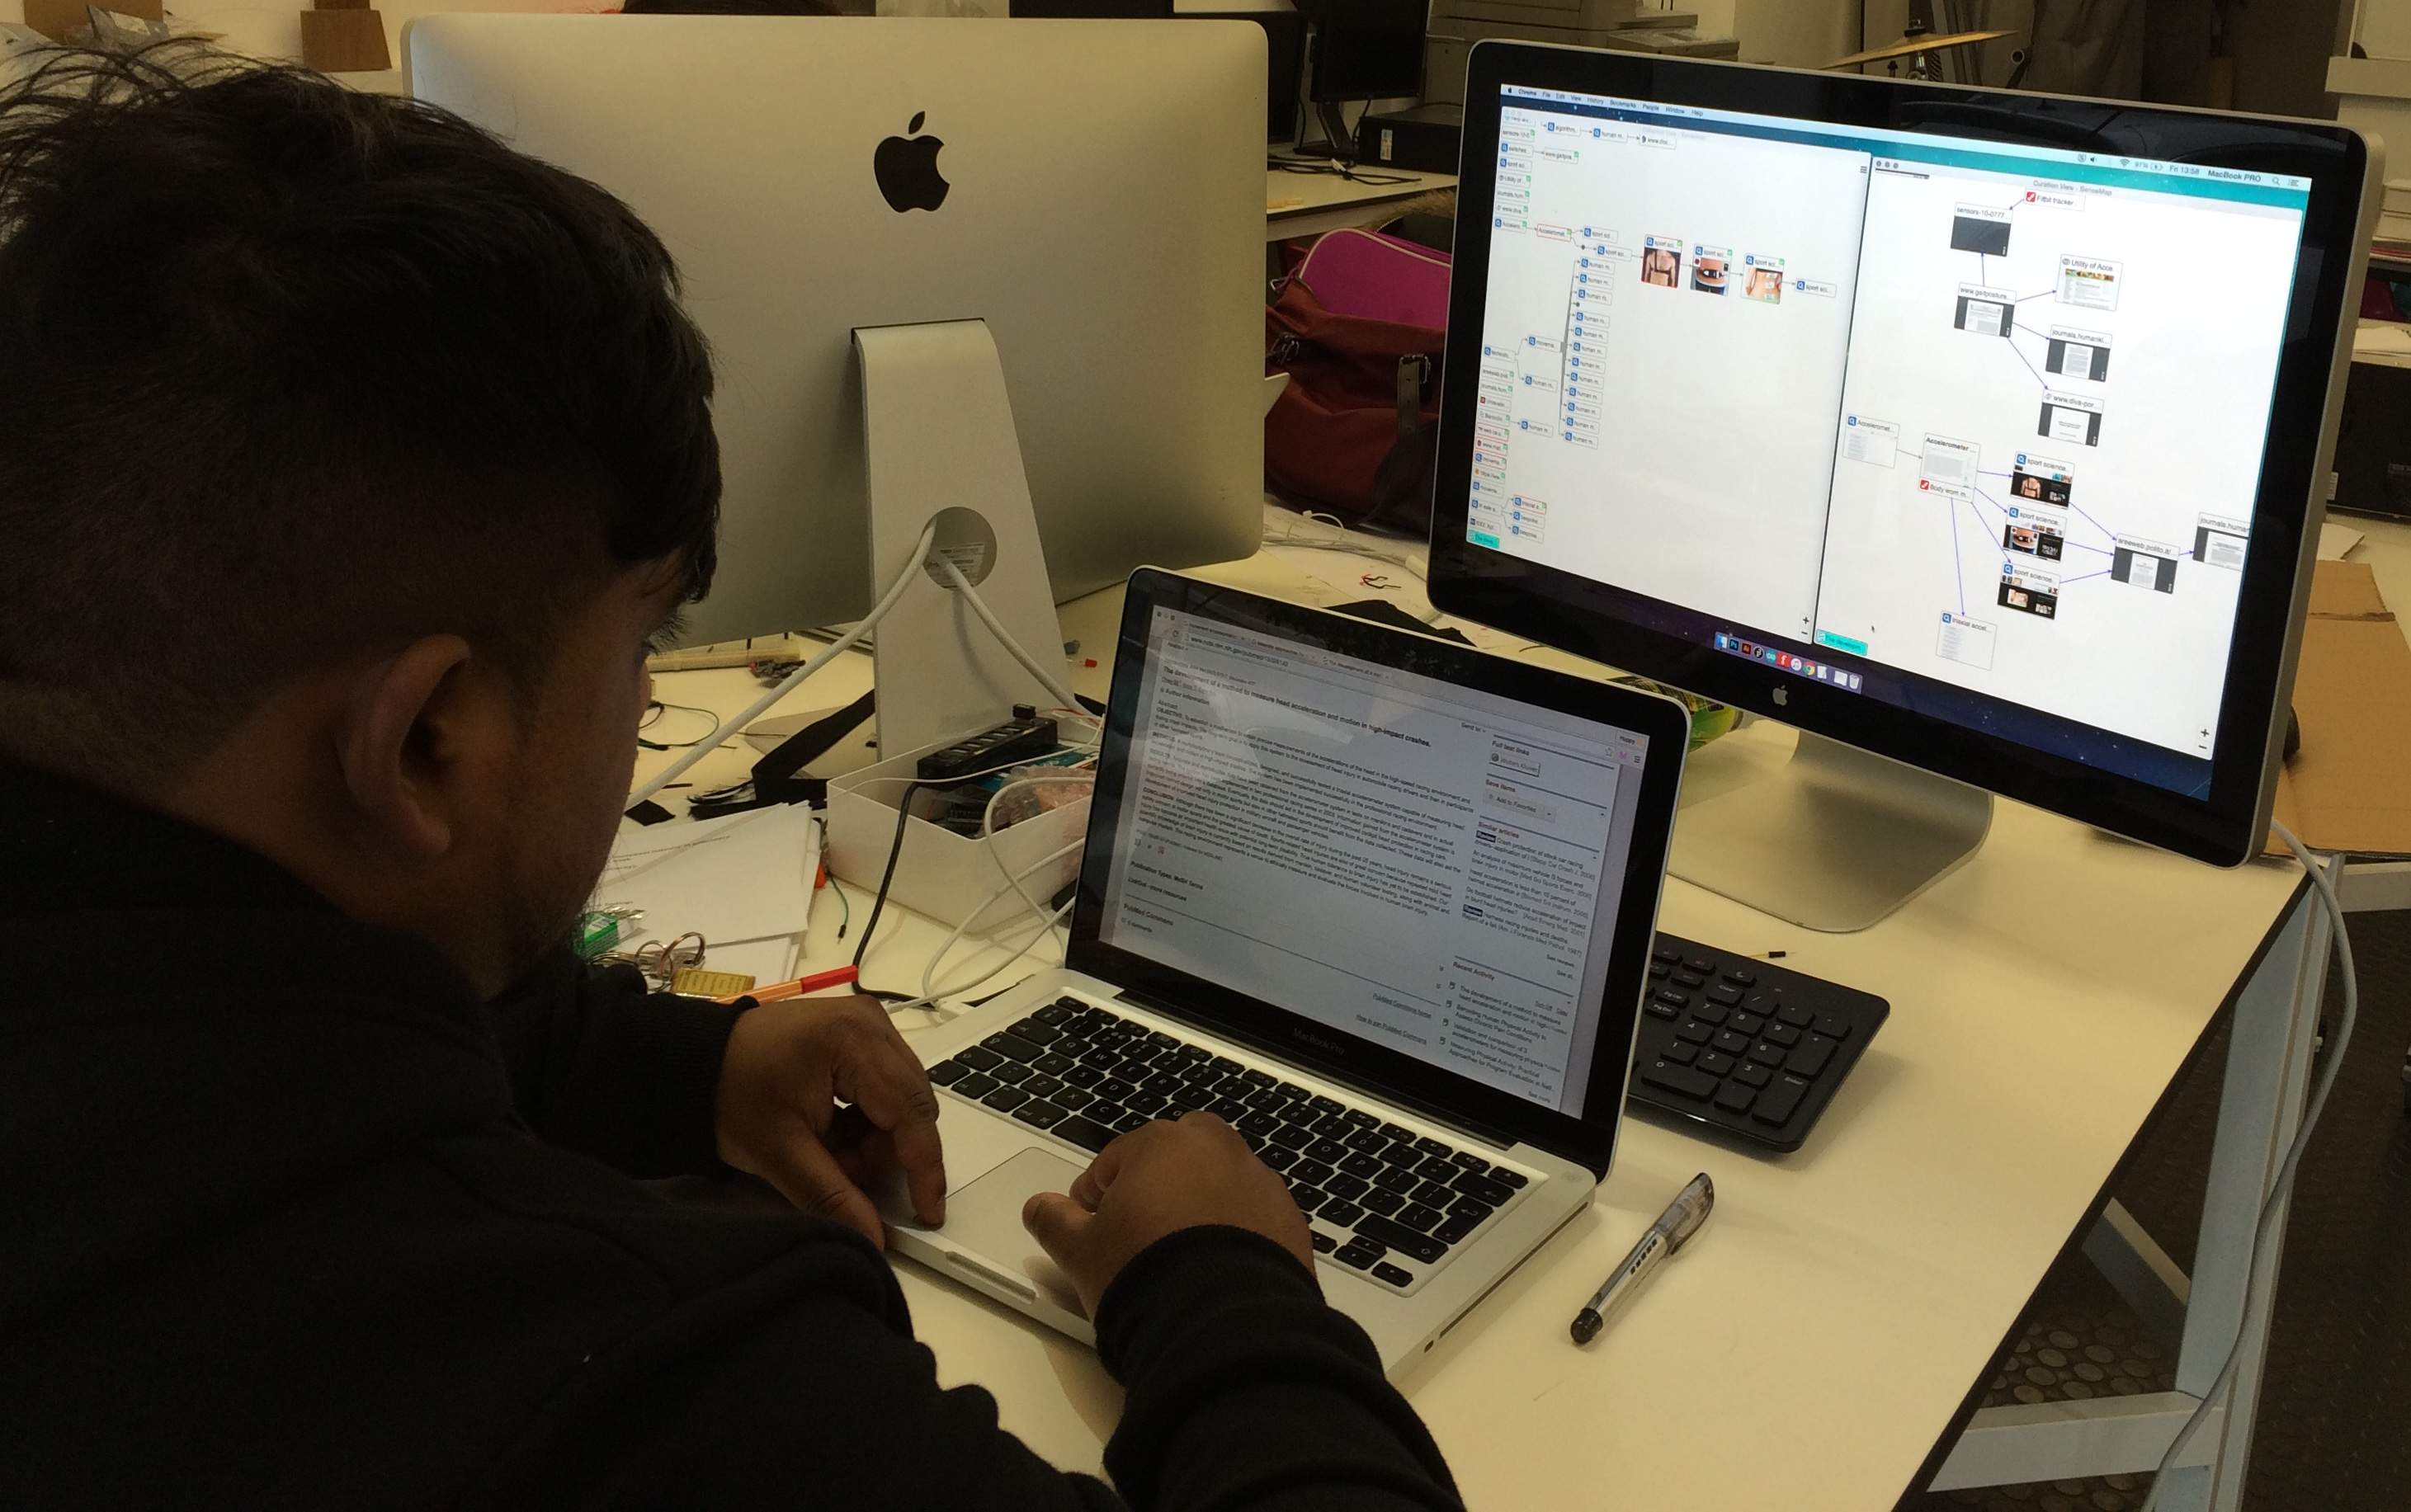
\includegraphics[width=\linewidth]{evaluation-two-monitors.jpeg}
	\caption[P5 with two monitors]{P5 with two monitors, comfortably interacting with all three views of SenseMap.}
	\label{fig:evaluation-two-monitors}
\end{figure}

\textbf{Negative: P3, P4}. Both of them reverted to full-screen browser windows and expressed a strong preference for this. P3 ignored the history map after losing reassurance that the tool could support him in his task. P4 reset the browser view to full screen, ignored the history map, and then lost track of the meaning of the collection when she returned to it.

\paragraph{F3 -- Keeping Track}
Did the participant understand and keep track of the building collection in the history map?

\textbf{Positive: P1, P2, P3, P5}. P5 had a second monitor attached so he could see the history map at all times. He said that the tool really began to make sense for him when he connected the second monitor and he felt his pace increased. P1 said he had resized the browser to full screen and ignored the history map, but it continued to make sense to him. He characterized his use as having regular periods of interaction with the history map rather than regular observation of it building up. P3 maintained track in the early phases of the task and did extensive preparation for curation by minimizing nodes to keep track and guide his searches.

\textbf{Negative: P4}. Early in the task, P4 decided to reset the browser window to full-screen and to ignore the history map. When she returned to the history map she found she had lost track and did not satisfactorily regain it throughout the rest of the task.

\paragraph{F4 -- Trust}
Did the participant maintain trust in the tool throughout the process? Were they confident that nodes were appearing in the correct relationship and with the correct links to other nodes? Did they understand these relationships when looking at the history map?

\textbf{Positive: P1, P2, P5}. They all expressed feelings of trust in the tool and were able to confidently shift their sensemaking activity focus from collections of tabs to the history and knowledge maps.

\textbf{Negative: P3, P4}. P3 had been managing the history map, but lost trust in the tool as they began to question the position and relationship of nodes generated in the history map to other nodes in that map. P4 lost trust in the tool as he could not understand the relationship of the nodes in the history map.

\paragraph{F5 -- Reassurance}
Was the participant reassured that the tool would provide sufficient support to complete the task? Did the participant believe that the added value in organization of information sources would outweigh the effort?

\textbf{Positive: P1, P2, P5}. P2 referred to the history map and the knowledge map as a good aide memoir allowing him to check completeness and to guide further searches. He felt reassured enough by the growing history map to close browser tabs. In his normal practice, he often created reports based on his tab sets to communicate his findings. He was confident and enthusiastic that SenseMap could remove this burden. P1 saw much potential in the tool and asked if he could use it for a big design project that he would be competing in the following year. He had regular interaction with the history map and used it the most to revisit previous sources of information clicking on nodes in the history map (44\% of web browser page reloads). P5 described the history map as ``my thinking'' and the knowledge map as ``a neater view of my thinking''. His reference to having a ``second brain'' was clearly reassuring to him.

\textbf{Negative: P3, P4}. P3 was initially reassured by the tool. However, this reassurance diminished over time as he began to feel that the management of the collection was impeding his ability to complete the task and gradually lost interest in the collection view, reverting to his typical sensemaking methods using tabs and a full screen browser window. P4 had lost track and no longer felt reassured that the tool could support her activity.

Table \ref{table:features} summarizes the status of each feature for all participants.

\begin{table}
\centering
\sffamily\small
\caption{Qualitative features derived  from all participants.}
\label{table:features}
\begin{tabular}{cccccc}
	\toprule
	 & \textbf{Comm.} & \textbf{Window} & \textbf{Keeping Track} & \textbf{Trust} & \textbf{Reassurance}\\
	\midrule
 				P1 & \cmark & \cmark & \cmark & \cmark & \cmark \\
 				P2 & \cmark & \cmark & \cmark & \cmark & \cmark \\
 				P3 & & & \cmark  &  \\
 				P4 & & & &  &  \\
 			    P5 & \cmark & \cmark & \cmark & \cmark & \cmark \\
	\bottomrule
\end{tabular}
\end{table}

\subsection{Discussion}
We roughly assess the quality of the sensemaking outcome for each participant. The metric is based on the number of relevant sources that the participants found and the coherence in the organization of these sources. Both factors are assessed by a senior interaction designer who is the head of the project that the participants are involving. The coherent organization is reflected through both the knowledge map and the explanation of such structure if it was hidden in the participant's mind. \autoref{table:quality} summarizes the assessment result.

\begin{table}
\centering
\sffamily\small
\caption{Quality of sensemaking outcome of participants.}
\label{table:quality}
\begin{tabular}{ccc}
	\toprule
	\textbf{Participant} & \textbf{Number of relevant sources} & \textbf{Coherence of schema} \\
	\midrule
 		P1 & 6 & good \\
 		P2 & 13 & very good \\
 		P3 & 7 & poor \\
 		P4 & 5 & poor \\
 		P5 & 9 & satisfactory \\
	\bottomrule
\end{tabular}
\end{table}

The most notable pattern we discovered in both quantitative and qualitative features is a clear division of participants into two groups. One group (P1, P2 and P5) highly engaged with the  curation process and were positive in all five qualitative features. Whereas, the other group (P3 and P4) engaged weakly with curation and were negative in almost all five qualitative features. This division was also true in the quality of the sensemaking outcome: P1, P2 and P5 found more relevant sources than P3 and P4 (note that P1 only spent half of the time that other participants) and structured them in a more coherent schema. This pattern may suggest an almost linear process relating all these features. Users who were able to manage tool windows were also able to keep track of the development of the history map, allowing them to trust that the tool would work properly and reassure that the tool would provide sufficient support to complete the task. Eventually, they were able to communicate their findings effectively and had more successful outcomes.

Next, we will discuss two lessons we learned in this evaluation.

\subsubsection{Engagement}
High engagement with the browser view, the history map and the knowledge map could lead to a positive outcome. All three participants who had positive outcomes achieved this engagement either through having multiple monitors that display all three windows simultaneously (P5) or having the skill and willingness to regularly switch between them (P1 and P2). The challenge is how to design a more space-efficient history map to be displayed side-by-side with the browser view.  Alternatively, the history map could be invisible while users are focusing on the browser view, but provide sufficient feedback to help them keep track of the map construction. Also, a visual summary of what has happened since the last time the history map is active could help users to catch up more quickly.

Another factor could impede user understanding of the history map is the complexity of the map itself.  As discussed in \autoref{sub:sm-layout}, the history map uses a compact tree layout to produce a tidy visualization. However, as the exploration progresses, the visualization expands and may not fit into the display area, requiring users to manually zoom and pan. To address this issue, we need to ensure the active part of the map be always visible to users by automatically panning the visualization. Another approach is to automatically summarize or condense the inactive part of the map, which could be measured by the spatial or temporal distance to the most active ones. All these actions need to be performed with smooth transitions to maintain user awareness.

Besides technical limitation, low user engagement could be related to a cognitive aspect~\cite{OBrien2008,Peters2009}. It is essential to investigate when and why the participants lost their engagement. Was it because the participants did not understand how information was represented? Was it because the information was represented in a too complex way that caused cognitive overload? Or did the participants understand the visual designs but found the interface too cumbersome to interact with? Having a clearer understanding of why the participants lost their engagement will help design a more useful interface.

\subsubsection{Trust and Reassurance}
It is essential to maintain the trust and the reassurance of users with the tool, enabling them to continue curating their collected information and gaining benefit from the curation process. Our initial interviews identified user anxiety over retaining and organizing tabs. Losing collections of tabs is seen as a serious event. SenseMap requires users to trust that it is recording their browsing activities accurately and in a manner that they can continue to understand throughout the sensemaking process. In essence, users pass control over the collection phase of their sensemaking process to the tool (trust) and curate this collection in ways that aim to provide enhanced ways to understand and present this knowledge (reassurance).

SenseMap is designed to support and augment browser-based online sensemaking and thus requires a change in practice from sensemaking through a collection of browser tabs to sensemaking by engaging with the history and knowledge maps. Our data shows that all participants who had a positive engagement profile were able to make the necessary practice change, were reassured by the tool's ability to support their work and maintained trust in it, and eventually produced successful outcomes. In the negative cases, the two participants were either unable or unwilling to change their practice. This insight suggests that spending time in curation is likely worth the effort; however, users may only curate if they trust and reassure that the tool will help them. The challenge is how to improve trust and reassurance through both the construction process and presentation of our history map. A think-aloud study of user's responses to history map construction would be an obvious next step that could stimulate alternative design proposals.

\paragraph{Opportunities for Further Improvement}
The evaluation shows that SenseMap provides useful sensemaking support for users in a 2-hour-long session. However, in the real world, a sensemaking task can be split  into small chunks and spanned multiple days or even weeks. Because SenseMap is implemented as a Chrome extension, this gives us an opportunity to conduct a longer term and larger scale study to gain a better understanding of SenseMap's use.

Finally, all participants mentioned that they would like to be able to add notes to the knowledge map; one had even invented a way to do this himself using search terms. They would like to be able to label clusters and links to those clusters and also provide explanations about hypotheses and recommendations. This would also help users record their internal knowledge prior to the tasks.